\section{Kreise}

\subsection{Bestimmen sie eine Funktion für die angegebenen Kreise}

\begin{enumerate}
\item
\begin{center}
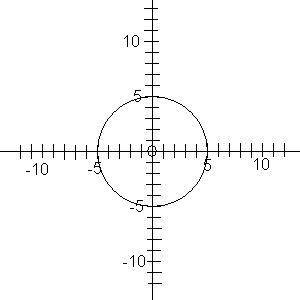
\includegraphics[width=0.5\textwidth]{img/Aufgaben/Kreise/K1.jpg}
\end{center}

%\newpage
 
\item
\begin{center}
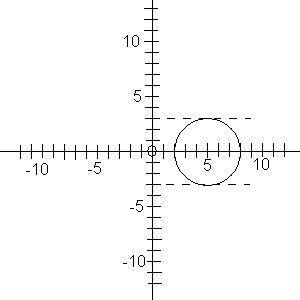
\includegraphics[width=0.5\textwidth]{img/Aufgaben/Kreise/K2.jpg}
\end{center}

\item
\begin{center}
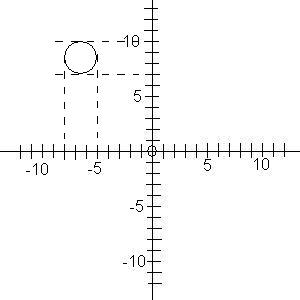
\includegraphics[width=0.5\textwidth]{img/Aufgaben/Kreise/K3.jpg}
\end{center}

%\newpage
\item
\begin{center}
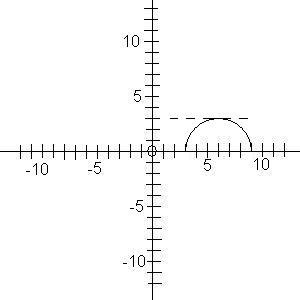
\includegraphics[width=0.5\textwidth]{img/Aufgaben/Kreise/K4.jpg}
\end{center}

\item
\begin{center}
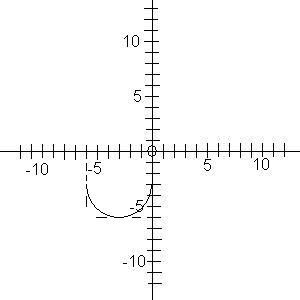
\includegraphics[width=0.5\textwidth]{img/Aufgaben/Kreise/K5.jpg}
\end{center}
\end{enumerate}
%\newpage

\section{Ungleichungen}

Für alle Aufgaben gilt grundsätzlich:
$ x, y, z \in \mathbb{R} $ sind Variable
$ a, b, c \in \mathbb{R} $ sind feste Parameter

\subsection{Ungleichungen mit einer Variablen}

%\LARGE{
Lösen Sie die folgenden Ungleichungssysteme analytisch:
%}\normalsize

\begin{enumerate}
\item
\[(x \ + \ 1)(x \ - \ 1) \ \leq 0\]
\[\sqrt x \geq 1 \]

%\item
%\[(x \ + \ 2)^2 \ + \ \frac 1 {1 \ + \ x} < x^3 \ + \ 3x^2 \ + \ 4x  + \ 3 \]

\item
\[ \sqrt{\frac 1 2 x^3 \ + \ 2x^2 \ + \ \frac {21} 8 x \ + \ \frac 9 8} \ < \ \sqrt{\frac 1 2 x^2 \ + \ \frac 3 2 x \ + \ \frac 9 8 } \]

\item
\[\frac 1 2 x^2 \ - \ 1 \ > \ 0\]

\item
\[x^3 \ + \ 3x^2 \ - \ 4 \ > \ 0\]

\item
\[x^3 \ + \ 3x^2 \ + \ 3x \ + \ 1 < 0\]

\item
\[x^6 \ - \ 6x^5 \ + \ 15x^4 \ - \ 20x^3 \ + \ 15x^2 \ - \ 6x \ + \ 1 \ \leq \ 0\]

\item
\[\frac 1 2 x^2 \ - \ 8 \ > \ 0\]
\[-3(x \ - \ 1)^2 \ + \ 12 \ > \ 0\]

\item
\[(x^2 \ - \ 2)(x \ + \ 1) \ \geq \ 0\]

\item Geben Sie die Lösungsmenge des Ungleichungssystem in Abhängigkeit von $ a $ an.
\[ax^2 \ > \ 0\]
\[\frac 1 2 x \ + \ 1 > 0\]

\item Geben Sie die Lösungsmenge des Ungleichungssystem in Abhängigkeit von $ a $ an.
\[x^2 \ + \ a \ > \ 0\]
\[\frac 1 2 x \ + \ 1 \ > \ 0\]

\item Geben Sie die Lösungsmenge des Ungleichungssystem in Abhängigkeit von $ a $ an.
\[-x^2 \ + \ a \ < \ 0\]
\[x \ + \ a \ < \ 0\]

\item Geben Sie die Lösungsmenge des Ungleichungssystem in Abhängigkeit von $ a $ an.
\[4x^2 \ - \ 2ax \ + \ \frac 1 4 a^2 \ \geq \ 0\]

\item
\[x^3 \ + \ x^2 \ - \ 2x \ \geq \ 2\]

\item
\[(x \ - \ 1)^2 \ - \ 4 \ < \ 0\]
\[-(x \ + \ 1)^2 \ + \ 4 \ > \ 0\]

\item
\[\sqrt {(x-1)} \ \geq \ 0\]
\[- \frac 1 4 x \ + \ 4 \ < \ 0\]

\item
\[x^4 \ - \ 16 \ \leq \ 0\]
\[x^3 \ + \ 1 \ \geq \ 0\]

\end{enumerate}
\newpage

\subsection{Ungleichungen mit mehreren Variablen}

%\LARGE{
Lösen Sie folgende Ungleichungssysteme graphisch:
%}\normalsize

\begin{enumerate}
\item
\[x^2 \ + \ y^2 \ < \ 25 \]
\[\frac 1 2 x \ + \ \frac 5 2 \ > \ y \]
\[-x \ - \ 5 \ < \ y \]

\item
\[- x^2 \ + \ 5 \ < \ y \]
\[x(x \ - \ 3)^2 \ > \ y \]
\[-x \ - \ 2 \ > \ y \]

\item
\[3x^2 \ - \ 3x \ - \ 10 \ < \ -4 \ + \ y \]
\[y \ \leq \ \frac 1 2 \]

\item
\[ y \ < \ \frac {2x^2 \ + \ 3x \ + \ 4} {- x^4 \ - \ 2x^3 \ - \ x^2 \ + \ 4x \ + \ (2x \ + \ x^2)^2} \]
\[- \frac 1 x \ < \ y \]
\[- ( \frac 1 {\sqrt 2} x )^2 \ < \ y \ - \ \frac 1 2 x^2 \ + \ \frac 1 2 x \ + \ 2 \]
\[y \ + \ x \ - \ 2 \ < \ 0 \]

\item
\[\frac 1 2 x^2 \ - \ 3x \ \leq \ y\]
%\[\frac 4x^3 \ + \ 2x^2 \ - \ \frac 13 4 x \ \geq \ y\]
\[y \ \leq \ -x\]
\[17x^3 \ - \ \frac 1 2 \ = \ y\]

\item
\[ y \ + \ \sqrt {\frac {x^3 \ + \ x^2 \ - \ x \ - \ 1} {x \ - \ 1}} \ > \ 0 \]
\[ \frac 2 {20} x \ - \ \frac 1 3 y \ + \ \frac 3 {12} \ < \ 0\]

\item
\[\frac 1 2 x \ - \ 2 < y\]
\[\frac 1 2 x \ + \ 2 > y\]
\[2 x \ - \ 4 < y\]
\[2 x \ + \ 4 > y\]
\[- \frac 1 2 x \ - \ 2 < y\]
\[- \frac 1 2 x \ + \ 2 > y\]
\[-2 x \ - \ 4 < y\]
\[-2 x \ + \ 4 > y\]

\item
\[|(x^2 \ + \ (y \ - \ 1)^2| \ = \ 4 \]
\[x \ \geq \ y \]

\item
\[((\sin x) \ + \ \frac 1 2)^2 \ - \ \frac 3 4 \ - \ y \ - \ (\sin x)^2 \]
\[\cos (x \ + \ \frac {\pi} 2 ) + \ \frac 1 2 \ < \ y \]

\item
\[| \frac 1 x| \ > y \]
\[- \frac {1 \ + \ 7x^2} {x^2 y} > \ - \frac {y \ + \ 7} y\]
\[|x| + y < 5\]

\item
\[4x^2 \ + \ y^2 \ <= \ 16\]
\[x^2 \ + \ 4y^2 \ <= \ 16\]

\item
\[(y \ - \ 2)^2 \ < \ 4 - (x \ - \ 2)^2\]
\[y -2 < 0\]
\[-|x \ - \ 2| \ + \ 2\ < \ y\]

\item Berechnen Sie für die Ungleichung den Flächeninhalt der Lösungsmenge:
\[ (2y \ - \ 3)^2 \ + \ (3y \ + \ 2)^2 \ + \ y \ - \ 10 \ \geq \ | \frac {4x \ + \ 4 (\frac 1 2 x \ - \frac 3 2 )^2 \ - \ 9} x | \ + \ 13y^2 \]
\[y \ \leq \ -1\]

\item Berechnen Sie für das Ungleichungssystem den Flächeninhalt der Lösungsmenge:
\[f : x^2 \ - \ 4x \ + 4 \ + \ y^2 \ - \ 2y \ + \ 1 \ \geq \ 1 \]
\[g : (x \ - \ 2)^2 \ + \ (y \ - \ 2)^2 \ \leq \ 4 \]
\[h : (x \ - \ 2)^2 \ + \ (y \ - \ 3)^2 \ \geq \ 1 \]

\item
Für welches a ist der Flächeninhalt der Lösungsmenge $ = 2 $ ?
\[y \ \geq \ 2\]
\[-|x| \ + \ a \ \leq \ y\]

\item
Bestimmen Sie ein $a$ und ein $b$, für das der Flächeninhalt der Lösungsmenge $ 2 \pi $ ergibt!
\[- \frac 1 3 x \ \leq y \ - \ 2\]
\[(x+ \frac 1 4 b)^2 \ + \ (y \ - \ \frac 3 2 a)^2 \ \leq \ a^2\]

\item Beschreiben sie die Lösungsmenge des Ungleichungssystems:
\[x^2 \ + \ y^2 \ + \ z (z \ + \ 2) \ < \ 8 \]
\[x \ \leq \ 0 \]
\[y \ \leq \ 0 \]

\item Beschreiben sie die Lösungsmenge des Ungleichungssystems:
\[(x \ - \ 2 \sqrt 3)^2 \ + \ (x \ - \ 2 \sqrt 3)^2 \ + \ (z \ - \ 2 \sqrt 3)^2 \ \leq \ 36\]
\[(x \ + \ 2 \sqrt 3)^2 \ + \ (x \ + \ 2 \sqrt 3)^2 \ + \ (z \ + \ 2 \sqrt 3)^2 \ \leq \ 36\]

\end{enumerate}
